\label{theory}
\chapter{Theory}

Here we present and critically investigate \textit{proof with and without probabilities}. \citet{verheijProofProbabilities2017} formally defines the notion of a \textit{case model} and three different notions of arguments.

\section{Case models}

\begin{figure}[htb]
        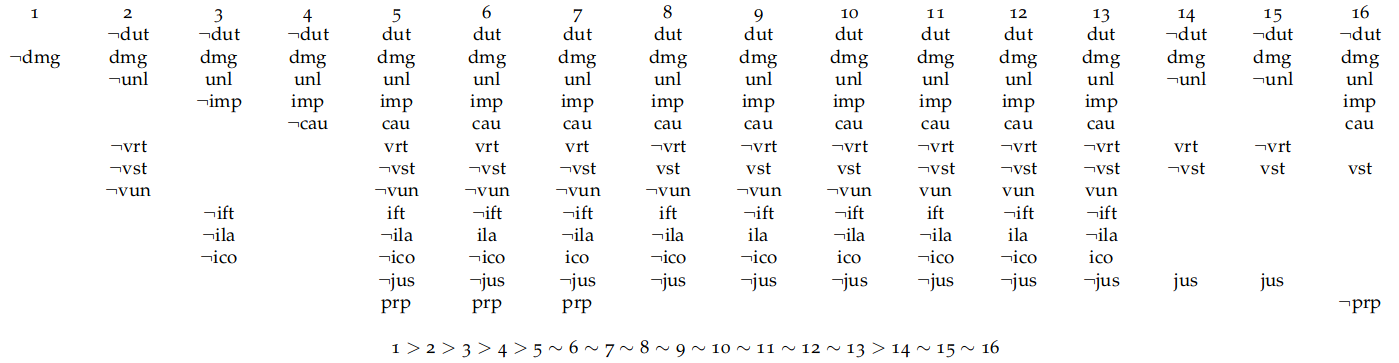
\includegraphics[width=\textwidth]{images/casemodel.png}
        \caption{Case model for Dutch law of unlawful acts. From \citet[fig.~23]{verheijArgumentsGoodArtificial2018}.}
        \label{fig:casemodel}
\end{figure}

A case model is a set of weakly ordered \textit{cases}, where each case is distinguished by the propositions that follow from it. We can alternatively define a case as the most general proposition which entails the propositions that follow from the case. 

For our purposes, we can restrict the definition of a case by demanding that it consists of a conjunction of literals. Then, we deal with cases that contain disjunctions of propositions by splitting them into multiple cases. This way, we arrive at a boolean (propositional) representation that is suitable for machine learning. We do this by interpreting a scenario as a data point in the training data.

One challenge is how to derive the preference relation over cases from the training data. The preference relation is relevant for identifying presumptively valid arguments. One approach here is the following: When we test whether an argument with a specific set of literals in the conclusion is presumptively valid, we aggregate the training data by the set of attributes that corresponds to the set of literals in the conclusion. We then take the count how many cases have been aggregated into one single case as an indication of how preferred this case is. 

\label{sec:arguments}
\section{Arguments}

\begin{figure}[htb]
        \centering
        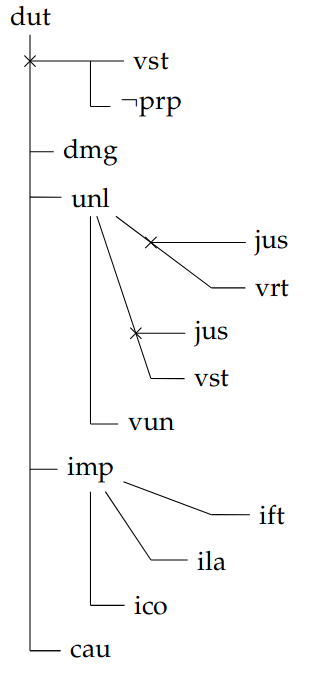
\includegraphics[width=0.15\textwidth]{images/argument.png}
        \caption{Argument structure (right) for Dutch law of unlawful acts. From \citet[fig.~5]{verheijArgumentsGoodArtificial2018}.}
        \label{fig:argument}
\end{figure}

In the context of this research project, the notions of conclusive and of presumptively valid arguments are interesting. The notion of a coherent argument is only interesting in so far as it is a condition for the two other types of arguments. 

\subsection*{Conclusive arguments}
An argument is \textit{conclusive} according to \citet{verheijProofProbabilities2017} if the conclusion is true in every case where the premises are true.

This raises the question whether an argument that is \textit{conclusive} in the sense of \citet{verheijProofProbabilities2017} is also conclusive in the sense of everyday language. There is no formal requirement on case models that they need to be exhaustive. Thus, we can imagine that in the real world (though not in the case model) the premises of an argument may hold and the conclusions may simultaneously not hold, but it would still be \textit{conclusive}  in the sense of \cite{verheijProofProbabilities2017}, just because this real world case is not included in the case model. Hence, the notion of an argument being \textit{conclusive} is misleading to a certain extent. We can fix this by adding the assumption that the case model exhaustively represents all the cases that hold in the real world; this may well be an implicit assumption of the original approach. 

When applying the approach to machine learning, the problem is anyway that the training data will normally never contain exhaustive data, and the idea of deriving conclusive arguments is vain -- consider the problem of induction. To get a probabilistic idea, we can utilize the idea of \textit{Bayesian smoothing}, which is epistemologically quite attractive. Bayesian smoothing in its standard variant of \textit{1-smoothing} states that the probability of an event that occurs $k$ times in a data set of size $n$ is not $\frac{k}{n}$, but rather $\frac{k}{n+1}$. (This is for binary data without prior probabilities only, and can be adjusted otherwise towards \textit{k-smoothing} or similar.) A \textit{conclusive} argument in the sense of the definition, then, is only valid probabilistically, resembling a strong presumptively valid argument.

\subsection*{Presumptively valid arguments}

An argument is \textit{(presumptively) valid} if the conclusion is true in the most likely or most preferred case in which the premises hold. Presumptively valid arguments are most interesting in the context of this project, since (a) they can have exceptions and are thus very much like human arguments, which is desirable from an explainable AI perspective, and (b) due to the strong conditions there will usually be only very few conclusive arguments in real world data, and the bulk of the arguments will be presumptively valid only. 